

\chapter{函数}\label{chapter:functions}


本章讨论从张量到其他张量的一般函数。
它们虽然不如线性函数优雅，却对许多应用都很重要，例如神经网络中的非线性。
主要目标是让向量链式法则变得直观且易于应用，不过我们也会讨论 Taylor 级数、行列式和其他主题。

当函数会沿某些维度广播时，向量函数的标准记号可能相当含糊。
如果 $x\in\R^n$ 是一个向量，那么 $f(x)$ 到底是独立作用在 $x$ 的每个元素上，还是把整个向量作为输入，并不清楚。
借助张量图，我们可以显式画出 $x$ 的哪些边进入 $f$、哪些边不进入，从而澄清这种区别。
我们使用记号
%If the result of $f(x)$ is itself a vector $\in\R^m$, we can write
\tikz[baseline=-.25em, inner sep=2pt]{
   \draw[->] (.5,0) node[right]{$x$} -- node[above, font=\tiny]{$n$} (0,0) node(f)[left]{$f$};
   \draw (f) -- ++(-.5,0) node[midway, above, font=\tiny] {$m$};
}
表示 $f$ 是从 $\R^n$ 到 $\R^m$ 的函数。
如果 $f$ 是逐元素函数，则写作
$(\tikz[baseline=-.25em, inner sep=2pt]{
   \draw[->, densely dotted] (.3,0) node[right](x){$x$} -- (0,0) node(f)[left]{$f$};
   \draw (x) -- ++(.5,0) node[midway, above, font=\tiny] {$n$};
}) \in \R^n$.
我们总是假设函数边（箭头边）先于普通边缩并。
如果想表达别的内容，例如 $f(Mx)$，可以使用括号：
\tikz[baseline=(f.base), inner xsep=2pt, inner ysep=0pt]{
   \node (f) at (0,0) {$f$};
   \draw (f) -- ++(-.5,0);
   \node (group) at (1.5,0) {$(
      \tikz {
         \node (M) at (0.5,0) {$M$};%
         \draw (0,0) -- (M) -- ++(.5,0) node[right]{$x$};%
      }%
      )$
   };
   \draw[->] (group) -- (f);
}.
再看一些例子会更有帮助：
%In the examples below, $x\in \R^n$:
\vspace{-1.5em}
\begin{center}
\begingroup
\renewcommand{\arraystretch}{2.5}
\begin{tabular}[h]{cccc}
   $f : \mathbb R^n \to \mathbb R$
   & $f(x) \in \mathbb R$
   & \tikz[baseline=-.25em]{\draw[->] (.5,0) node[right]{$x$} -- node[above, font=\tiny]{$n$} (0,0) node[left]{$f$}}
   & （标量函数）
   \\
   $g : \mathbb R^n \to \mathbb R^m$
   & $g(x) \in \mathbb R^m$
   & \tikz[baseline=(x.base)]{
      \node (x) at (0,0) {$x$};
      \node (g) at (-.75,0) {$g$};
      \draw[->] (x) -- (g) node[midway, above, font=\tiny] {$n$};
      \draw (g) -- ++(-.5,0) node[midway, above, font=\tiny] {$m$};
   }
   & （向量函数）
   \\
   $h : \mathbb R \to \mathbb R$
   & $h(x) \in \mathbb R^n$
   & \tikz[baseline=(x.base)]{
      \node (x) at (0,0) {$x$};
      \node (h) at (-.75,0) {$h$};
      \draw[->, densely dotted] (x) -- (h);
      \draw (x) -- ++(.5,0) node[right, font=\tiny] {$n$};
   }
   & （逐元素函数）
   \\
   \makecell[c]{$u : \mathbb{R}^n \to \mathbb{R}^m$ \\ $v \in \mathbb{R}^m$}
   & $v^T u(x) \in \mathbb R$
   & \tikz[baseline=(x.base)]{
      \node (x) at (0,0) {$x$};
      \node (v) at (-.75,0) {$v$};
      \node (u) at (-1.5,0) {$u$};
      \draw[->] (x) -- (v) node[midway, above, font=\tiny] {$n$};
      \draw (v) -- (u) node[midway, above, font=\tiny] {$m$};
   }
   & （向量乘向量函数）
   \\
   \makecell[c]{$A : \mathbb R^n \to \mathbb R^{m\times n},$\\$v \in \mathbb R^n$}
   & $A(x)v \in \mathbb R^m$
   & 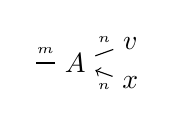
\begin{tikzpicture}[baseline=(A.base)]
      \node (A) at (0,0) {$A$};
      \draw (A) -- ++(-.5,0) node[midway, above, font=\tiny] {$m$};
      \node (x) at (.7,-.25) {$x$};
      \draw[->] (x) -- (A) node[midway, below, font=\tiny] {$n$};
      \node (v) at (.7,.25) {$v$};
      \draw (v) -- (A) node[midway, above, font=\tiny] {$n$};
   \end{tikzpicture}
   & （向量乘矩阵函数）
   \\
   \makecell[c]{$f : \mathbb R^d \to \mathbb R,$\\$X \in \mathbb R^{b\times d}$}
   & $f(X) \in \mathbb R^b$
   & 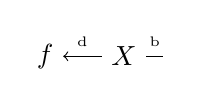
\begin{tikzpicture}[baseline=-.25em]
      \node (f) at (0,0) {$f$};
      \node (X) at (1,0) {$X$};
      \draw[->] (X) -- (f) node[midway, above, font=\tiny] {d};
      \draw (X) --  ++(.5,0) node[midway, above, font=\tiny] {b};
   \end{tikzpicture}
   & （向量函数，批量形式）
   \\
   \makecell[c]{$A : \mathbb R^{n\times m} \to \mathbb R,$\\$X \in \mathbb R^{n\times m}$}
   & $A(X) \in \R$
   & 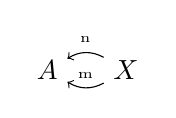
\begin{tikzpicture}[baseline=-.25em]
      \node (A) at (0,0) {$A$};
      \node (X) at (1,0) {$X$};
      \draw[->] (X) edge[bend right] node[midway, above, font=\tiny] {n} (A);
      \draw[->] (X) edge[bend left] node[midway, above, font=\tiny] {m} (A);
   \end{tikzpicture}
   & （矩阵输入函数）
   \\
   \makecell[c]{
      $f : \mathbb R^n\times \R^m \to \R^d$
      ,\\$u \in \mathbb R^{b\times n}
      , v \in \R^{b\times m}$
   }
   & $f(u, v) \in \R^{b \times d}$
   & 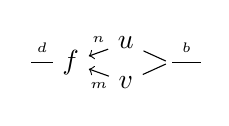
\begin{tikzpicture}[baseline=-.25em]
      \node (f) at (0,0) {$f$};
      \draw (f) -- ++(-.5,0) node[midway, above, font=\tiny] {$d$};
      \node (u) at (.7,.25) {$u$};
      \draw[->] (u) -- (f) node[midway, above, font=\tiny] {$n$};
      \node (v) at (.7,-.25) {$v$};
      \draw[->] (v) -- (f) node[midway, below, font=\tiny] {$m$};
      \node[inner sep=1pt] (d) at (1.25,0) {$\sbullet$};
      \draw (u) -- (d);
      \draw (v) -- (d);
      \draw (d) -- ++(.4,0) node[midway, above, font=\tiny] {$b$};
   \end{tikzpicture}
   & （两个输入，批量形式）
\end{tabular}
\endgroup
\end{center}

为了更具体一些，考虑几个熟悉的函数：
(1) 行列式函数 $\det : \mathbb R^{n\times n} \to \mathbb R$ 是一个标量函数，我们可以将它应用到一批矩阵上：
\tikz[baseline=(det.base), inner sep=2pt, every node/.append style={anchor=base}]{
      \node (det) {$\det$};
      \node[right=1.5em of det] (X) {$X$};
      \draw[->] (X) edge[bend right] node[midway, above, font=\tiny] {n} (det);
      \draw[->] (X) edge[bend left] node[midway, above, font=\tiny] {m} (det);
      \draw (X) -- ++(.5,0) node[right, font=\tiny] {$b$};
   }，结果得到一个向量 $\in\R^b$。
%
   (2)
   余弦相似度 $\mathrm{cossim} : \mathbb R^n \times \mathbb R^n \to \mathbb R$ 是一个标量函数，可以把它应用到两个向量上：
   \tikz[baseline=(cos.base), inner sep=2pt, every node/.append style={anchor=base}]{
      \node (cos) at (0,0) {$\mathrm{cossim}$};
      \node (u) at (1,.15) {$u$};
      \draw[->] (u) -- (cos) node[midway, above, font=\tiny] {$n$};
      \node (v) at (1,-.15) {$v$};
      \draw[->] (v) -- (cos) node[midway, below, font=\tiny] {$n$};
   }，结果得到一个标量 $\in\R$。
% 
   (3)
  如果逐元素幂函数 $\mathrm{pow}_n : \mathbb R \to \mathbb R$
      应用于两个向量，那么它们在 Hadamard 积下可以化简：
      \[
         \begin{tikzpicture}[baseline=(s.base), inner sep=2pt, every node/.append style={anchor=base}]
            \node (pown) {$\mathrm{pow}_n$};
            \node[right=1em of pown] (u1) {$u$};
            \node[below=.5em of pown] (powm) {$\mathrm{pow}_m$};
            \node[below=.5em of u1] (u2) {$u$};
            \draw (u1) edge[->, densely dotted] (pown);
            \draw (u2) edge[->, densely dotted] (powm);
            \node (s) at (1.5, -.25) {$\sbullet$};
            \draw (u1) -- (s);
            \draw (u2) -- (s);
            \draw (s) -- ++(.5,0);
         \end{tikzpicture}
         =
         \begin{tikzpicture}[baseline=(pow.base), inner sep=2pt, every node/.append style={anchor=base}]
            \node (pow) {$\mathrm{pow}_{n+m}$};
            \node[right=1em of pow] (u) {$u$};
            \draw (u) edge[->, densely dotted] (pow);
            \draw (u) -- ++(.5,0);
         \end{tikzpicture}
      \]

作为一个更进阶的例子，考虑 softmax 函数：
\tikz[baseline=(sm.base), inner sep=2pt, every node/.append style={anchor=base}]{
   \node (sm) {$\mathrm{softmax}$};
   \node[right=1em of sm] (x) {$x$};
   \draw[->] (x) -- (sm) node[midway, above, font=\tiny] {$d$};
   \draw (sm) -- ++(-1,0) node[midway, above, font=\tiny] {$d$};
}.
可以把它写成如下初等函数组合：
\[
   \mathrm{softmax}(x)
   =
   \frac{\mathrm{exp}(x)}{\mathrm{sum}(\mathrm{exp}(x))}
   =
   \begin{tikzpicture}[baseline=-1em, every node/.append style={anchor=base}]
      \node (ex1) at (0,0) {$\mathrm{exp}$};
      \node (x1) at (1,0) {$x$};
      \draw (ex1) edge[<-, densely dotted] (x1);
      \draw (x1) -- ++(.5,0);
      % Second row
      \node (pow) at (-1,-.6) {$\mathrm{pow}_{-1}$};
      \node[right=1em of pow] (b1) {$($};
      \node[right=0em of b1] (exp2) {$\mathrm{exp}$};
      \node[right=1em of exp2] (x2) {$x$};
      \node[right=1em of x2, inner sep=1pt] (s) {$\sbullet$};
      \draw (x2) edge[->, densely dotted] (exp2);
      \draw (b1) edge[->, densely dotted] (pow);
      \draw (x2) -- (s);
      \node[right=0em of s] (b2) {$)$};
   \end{tikzpicture}
\]
一开始它看起来有点复杂，但我们可以逐步拆开：
$(\tikz[baseline=(ex1.base), every node/.append style={anchor=base}]{
   \node (ex1) at (0,0) {$\mathrm{exp}$};
   \node (x1) at (1,0) {$x$};
   \draw (ex1) edge[<-, densely dotted] (x1);
   \draw (x1) -- ++(.5,0);
}) \in \R^n$ 是逐元素指数函数。
如果把它与 $\tikz[baseline=(s.base)] {
   \node[inner sep=1pt] (s) {$\sbullet$};
   \draw (s) -- ++(-.4,0);
}$ 缩并，就得到和 $s=\sum_i \exp(x_i)$。
最后，将 $\mathrm{pow}_{-1}$ 作用到 $s$ 上，并与指数函数相乘，就得到 softmax 函数。

有一种情况可能会稍显混乱：输出张量与输入张量的广播边发生缩并。
但只要记住先缩并函数边，一切就仍然成立。
例如，对于函数 $f : \R^n \to \R$ 和矩阵 $x \in \R^{m \times n}$：
\[
   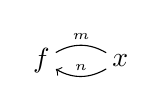
\begin{tikzpicture}[baseline=(f.base), inner sep=2pt]
      \node (f) {$f$};
      \node (x) at (1,0) {$x$};
      \draw (x) edge[bend right] node[midway, above, font=\tiny] {$m$} (f);
      \draw (x) edge[->, bend left] node[midway, above, font=\tiny] {$n$} (f);
   \end{tikzpicture}
   =
   \hspace{-2.3em}
   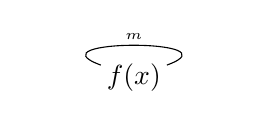
\begin{tikzpicture}[baseline=(f.base), inner sep=2pt]
      \node (f) {$f(x)$};
      \path (f) edge [out=160, in=20, looseness=3] node[midway, above, font=\tiny] {$m$} (f);
   \end{tikzpicture}
   \hspace{-2.3em}
   =
   \Tr(f(x))
   .
\]

\section{链式法则}
张量图最吸引人的特性之一，是链式法则在其中非常透明。对于两个函数
\(
   f: \mathbb{R}^m \to \mathbb{R} \quad \text{和} \quad v: \mathbb{R}^n \to \mathbb{R}^m,
\)
复合函数 $f\circ v: \mathbb{R}^n \to \mathbb{R}$ 只需把 $v$ 的输出送入 $f$，就可以画成图：
\[
   \tikz[baseline=(f.base), inner sep=2pt, every node/.append style={anchor=base}]{
      \node (f) {$f$};
      \node[right=1em of f] (v) {$v$};
      \node[right=1em of v] (x) {$x$};
      \draw[->] (x) -- (v);
      \draw[->] (v) -- (f);
   }
\]
在传统记号中，链式法则写作
\(
   J_{f\circ v}(x)=\nabla f(v(x))\,J_v(x),
\)
其中 $J_v(x)$ 是 $v$ 的 Jacobian 矩阵，$\nabla f(v(x))$ 是 $f$ 在 $v(x)$ 处的梯度。
在张量图中，\emph{链式法则真的就是一条链！}
\[
   \begin{tikzpicture}[baseline=-1em, inner sep=1pt]
      \node (n0) {$f$};
      \node[below=1em of n0] (n1) {$v$};
      \node[below=1em of n1] (n2) {$x$};
      \draw[->] (n2) -- (n1);
      \draw[->] (n1) -- (n0);
      \drawellipse{0}{-.55}{.5}{1}{180/4}
   \end{tikzpicture}
   =
   \hspace{.5em}
   \begin{tikzpicture}[baseline=-1em, inner sep=1pt]
      \node[dn] (n0) {$f$};
      \node[below=1em of n0] (n1) {$v$};
      \node[below=1em of n1] (n2) {$x$};
      \node[right=1em of n0, dn] (n3) {$v$};
      \node[below=1em of n3] (n4) {$x$};
      \draw[->] (n2) -- (n1);
      \draw[->] (n1) -- (n0);
      \draw[->] (n4) -- (n3);
      \draw[d0] (n0) -- (n3);
      \draw[d0] (n3) -- ++(.5,0);
   \end{tikzpicture}
   \hspace{3em}
   \begin{tikzpicture}[baseline=-1em, inner sep=1pt]
      \node (n0) {$f$};
      \node[below=1em of n0] (n1) {$v$};
      \node[below=1em of n1] (n2) {$u$};
      \node[below=1em of n2] (n3) {$x$};
      \draw[->] (n3) -- (n2);
      \draw[->] (n2) -- (n1);
      \draw[->] (n1) -- (n0);
      \drawellipse{0}{-.75}{.5}{1.5}{180/4}
   \end{tikzpicture}
   =
   \hspace{.5em}
   \begin{tikzpicture}[baseline=-1em, inner sep=1pt]
      \node[dn] (n0) {$f$};
      \node[below=1em of n0] (n1) {$v$};
      \node[below=1em of n1] (n2) {$u$};
      \node[below=1em of n2] (n3) {$x$};
      \node[right=1em of n0] (n4) {$v$};
      \node[below=1em of n4] (n5) {$u$};
      \node[below=1em of n5] (n6) {$x$};
      \draw[->] (n3) -- (n2);
      \draw[->] (n2) -- (n1);
      \draw[->] (n1) -- (n0);
      \draw[->] (n6) -- (n5);
      \draw[->] (n5) -- (n4);
      \draw[d0] (n0) -- (n4);
      \drawellipse{.75}{-.55}{.5}{1}{180/4}
   \end{tikzpicture}
   =
   \hspace{.5em}
   \begin{tikzpicture}[baseline=-1em, inner sep=1pt]
      \node[dn] (n0) {$f$};
      \node[below=1em of n0] (n1) {$v$};
      \node[below=1em of n1] (n2) {$u$};
      \node[below=1em of n2] (n3) {$x$};
      \node[right=1em of n0, dn] (n4) {$v$};
      \node[below=1em of n4] (n5) {$u$};
      \node[below=1em of n5] (n6) {$x$};
      \node[right=1em of n4, dn] (n7) {$u$};
      \node[below=1em of n7] (n8) {$x$};
      \draw[->] (n3) -- (n2);
      \draw[->] (n2) -- (n1);
      \draw[->] (n1) -- (n0);
      \draw[->] (n6) -- (n5);
      \draw[->] (n5) -- (n4);
      \draw[->] (n8) -- (n7);
      \draw[d0] (n0) -- (n4);
      \draw[d0] (n4) -- (n7);
      \draw[d0] (n7) -- ++(.5,0);
   \end{tikzpicture}
\]
这清楚地符合经典口诀：“外层函数的导数乘以内层函数的导数”。
唯一需要细化的是，“外层函数”要通过求导产生的新边连接到“内层函数”。

也可以进一步把 \tikz[baseline=(f.base), inner sep=2pt]{\node[dn](f){$f$}; \draw[d0](f)--++(.6,0);} 简化成 \tikz[baseline=(f.base), inner sep=2pt]{\node(f){$f'$}; \draw(f)--++(.5,0);}，其中 $f'$ 是 $f$ 的导数。
例如，如果 $f$ 是 $\cos-$，那么 $f'$ 就是 $\sin-$。
不过，也可以继续保留带圈的 $f$，把它作为容易识别的导数符号。

\subsection{Hessian 链式法则}
当考虑二阶导数时，事情会变得更有意思。
使用标准记号，$f\circ v$ 的 Hessian 矩阵为
\[
H_{f\circ v}(x) = Dv(x)^T \cdot D^2f(v(x)) \cdot Dv(x) + \sum_{k=1}^d \frac{\partial f}{\partial u_k}(v(x)) \frac{\partial^2 v_k}{\partial x \partial x^T}(x).
\]
这个“Hessian 链式法则”用张量图推导要容易得多：
\begin{align*}
   \begin{tikzpicture}[baseline=-1em, inner sep=1pt]
      \node (n0) {$f$};
      \node[below=1em of n0] (n1) {$v$};
      \node[below=1em of n1] (n2) {$x$};
      \draw[->] (n2) -- (n1);
      \draw[->] (n1) -- (n0);
      \drawellipse{0}{-.55}{.5}{1}{180/4}
      \drawellipse{0}{-.55}{.7}{1.2}{180/4}
   \end{tikzpicture}
   &=
   \hspace{.5em}
   \begin{tikzpicture}[baseline=-1em, inner sep=1pt]
      \node[dn] (n0) {$f$};
      \node[below=1em of n0] (n1) {$v$};
      \node[below=1em of n1] (n2) {$x$};
      \node[right=1em of n0, dn] (n3) {$v$};
      \node[below=1em of n3] (n4) {$x$};
      \draw[->] (n2) -- (n1);
      \draw[->] (n1) -- (n0);
      \draw[->] (n4) -- (n3);
      \draw[d0] (n0) -- (n3);
      \draw[d0] (n3) -- ++(.5,0);
      \drawellipse{.4}{-.55}{1}{1.2}{180/4}
   \end{tikzpicture}
 \\&=
   \hspace{.5em}
   \begin{tikzpicture}[baseline=-1em, inner sep=1pt]
      \node[dn] (n0) {$f$};
      \node[below=1em of n0] (n1) {$v$};
      \node[below=1em of n1] (n2) {$x$};
      \node[right=1.5em of n0, dn] (n3) {$v$};
      \node[below=1em of n3] (n4) {$x$};
      \draw[->] (n2) -- (n1);
      \draw[->] (n1) -- (n0);
      \draw[->] (n4) -- (n3);
      \draw[d0] (n0) -- (n3);
      \draw[d0] (n3) -- ++(.5,0);
      \drawellipse{0}{-.55}{.5}{1.2}{180/4}
   \end{tikzpicture}
   +
   \hspace{.5em}
   \begin{tikzpicture}[baseline=-1em, inner sep=1pt]
      \node[dn] (n0) {$f$};
      \node[below=1em of n0] (n1) {$v$};
      \node[below=1em of n1] (n2) {$x$};
      \node[right=1.5em of n0, dn] (n3) {$v$};
      \node[below=1em of n3] (n4) {$x$};
      \draw[->] (n2) -- (n1);
      \draw[->] (n1) -- (n0);
      \draw[->] (n4) -- (n3);
      \draw[d0] (n0) -- (n3);
      \draw[d0] (n3) -- ++(.5,0);
      \drawellipse{1}{-.25}{.5}{.7}{180/4}
   \end{tikzpicture}
 \\&=
   \hspace{.5em}
   \begin{tikzpicture}[baseline=-1em, inner sep=1pt]
      \node[ddn] (n0) {$f$};
      \node[below=1em of n0] (n1) {$v$};
      \node[below=1em of n1] (n2) {$x$};
      \node[right=1em of n0, yshift=-1em, dn] (n3) {$v$};
      \node[below=1em of n3] (n4) {$x$};
      \node[right=1.5em of n3, yshift=1em, dn] (n5) {$v$};
      \node[below=1em of n5] (n6) {$x$};
      \draw[->] (n2) -- (n1);
      \draw[->] (n1) -- (n0);
      \draw[->] (n4) -- (n3);
      \draw[->] (n6) -- (n5);
      \draw[d0] (n0) -- (n3);
      \draw[d0] (n0) -- (n5);
      \draw[d0] (n3) -- ++(.5,0);
      \draw[d0] (n5) -- ++(.5,0);
   \end{tikzpicture}
   +
   \hspace{.5em}
   \begin{tikzpicture}[baseline=-1em, inner sep=1pt]
      \node[dn] (n0) {$f$};
      \node[below=1em of n0] (n1) {$v$};
      \node[below=1em of n1] (n2) {$x$};
      \node[right=1.5em of n0, ddn] (n3) {$v$};
      \node[below=1em of n3] (n4) {$x$};
      \draw[->] (n2) -- (n1);
      \draw[->] (n1) -- (n0);
      \draw[->] (n4) -- (n3);
      \draw[d0] (n0) -- (n3);
      \draw[d0] (n3) -- ++(.5,0);
      \draw[d0] ($(n3)+(.166,.15)$) -- ++(.4,0);
   \end{tikzpicture}
\end{align*}
如果继续以这种方式展开，就会看到更多函数的链式法则中存在一个简单模式：
\[\makebox[\textwidth][c]{
   \begin{tikzpicture}[baseline=-1em, inner sep=1pt]
      \node (n0) {$f$};
      \node[below=1em of n0] (n1) {$v$};
      \node[below=1em of n1] (n2) {$u$};
      \node[below=1em of n2] (n3) {$x$};
      \draw[->] (n3) -- (n2);
      \draw[->] (n2) -- (n1);
      \draw[->] (n1) -- (n0);
      \drawellipse{0}{-.75}{.5}{1.4}{180/4}
      \drawellipse{0}{-.75}{.6}{1.5}{180/4}
   \end{tikzpicture}
   =
   \hspace{.2em}
   \begin{tikzpicture}[baseline=-1em, inner sep=1pt]
      \node[ddn] (n0) {$f$};
      \node[below=1em of n0] (n1) {$v$};
      \node[below=1em of n1] (n2) {$u$};
      \node[below=1em of n2] (n3) {$x$};
      \draw[->] (n3) -- (n2);
      \draw[->] (n2) -- (n1);
      \draw[->] (n1) -- (n0);
%
      \node[right=1em of n0, yshift=-1em, dn] (n4) {$v$};
      \draw[d0] (n0) -- (n4);
      \node[below=1em of n4] (n5) {$u$};
      \node[below=1em of n5] (n6) {$x$};
      \draw[->] (n6) -- (n5);
      \draw[->] (n5) -- (n4);
      \node[right=1em of n4, dn] (u1) {$u$};
      \node[below=1em of u1] (u2) {$x$};
      \draw[->] (u2) -- (u1);
      \draw[d0] (n4) -- (u1);
      \draw[d0] (u1) -- ++(.5,0);
%
      \node[right=3.5em of n4, yshift=1em, dn] (n7) {$v$};
      \draw[d0] (n0) -- (n7);
      \node[below=1em of n7] (n8) {$u$};
      \node[below=1em of n8] (n9) {$x$};
      \draw[->] (n9) -- (n8);
      \draw[->] (n8) -- (n7);
      \node[right=1em of n7, dn] (u3) {$u$};
      \node[below=1em of u3] (u4) {$x$};
      \draw[->] (u4) -- (u3);
      \draw[d0] (n7) -- (u3);
      \draw[d0] (u3) -- ++(.5,0);
   \end{tikzpicture}
   +
   \hspace{.2em}
   \begin{tikzpicture}[baseline=-1em, inner sep=1pt]
      \node[dn] (n0) {$f$};
      \node[below=1em of n0] (n1) {$v$};
      \node[below=1em of n1] (n2) {$u$};
      \node[below=1em of n2] (n3) {$x$};
      \node[right=1.5em of n0, ddn] (n4) {$v$};
      \node[below=1em of n4] (n5) {$u$};
      \node[below=1em of n5] (n6) {$x$};
      \draw[->] (n3) -- (n2);
      \draw[->] (n2) -- (n1);
      \draw[->] (n1) -- (n0);
      \draw[->] (n6) -- (n5);
      \draw[->] (n5) -- (n4);
      \draw[d0] (n0) -- (n4);
      %
      \node[right=1em of n4, yshift=-1em, dn] (r1) {$u$};
      \node[below=1em of r1] (r2) {$x$};
      \draw[->] (r2) -- (r1);
      %
      \node[right=1.5em of r1, yshift=1em, dn] (r3) {$u$};
      \node[below=1em of r3] (r4) {$x$};
      \draw[->] (r4) -- (r3);
      %
      \draw[d0] (n4) -- (r1);
      \draw[d0] (n4) -- (r3);
      \draw[d0] (r1) -- ++(.5,0);
      \draw[d0] ($(r3)+(.166,.15)$) -- ++(.4,0);
   \end{tikzpicture}
   +
   \hspace{.2em}
   \begin{tikzpicture}[baseline=-1em, inner sep=1pt]
      \node[dn] (n0) {$f$};
      \node[below=1em of n0] (n1) {$v$};
      \node[below=1em of n1] (n2) {$u$};
      \node[below=1em of n2] (n3) {$x$};
      \node[right=1.5em of n0, dn] (n4) {$v$};
      \node[below=1em of n4] (n5) {$u$};
      \node[below=1em of n5] (n6) {$x$};
      \node[right=1.5em of n4, ddn] (n7) {$u$};
      \node[below=1em of n7] (n8) {$x$};
      \draw[->] (n3) -- (n2);
      \draw[->] (n2) -- (n1);
      \draw[->] (n1) -- (n0);
      \draw[->] (n6) -- (n5);
      \draw[->] (n5) -- (n4);
      \draw[->] (n8) -- (n7);
      \draw[d0] (n0) -- (n4);
      \draw[d0] (n4) -- (n7);
      \draw[d0] (n7) -- ++(.5,0);
      \draw[d0] ($(n7)+(.166,.15)$) -- ++(.4,0);
   \end{tikzpicture}
}\]
Yaroslav Bulatov 对 Hessian 链式法则以及如何在深度学习应用中高效求值写过大量文章。
感兴趣的读者可以参考他关于这一主题的博客文章。

\subsection{带广播的链式法则}
当链式法则应用于带广播的函数时，结果仍然遵循“外层导数乘以内层导数”的口诀，只是“乘”的含义扩展为对广播边取 Hadamard 积。
\[
   \includegraphics[width=.8\textwidth]{figures/chain_rule_broadcast.pdf}
\]

\subsection{多输入函数}
如果 $f : \mathbb{R}^m \times \mathbb{R}^n \to \mathbb{R}$ 是一个有两个输入的函数，那么 $f(x,y)$ 的导数就是 $\frac{\partial f}{\partial x}\partial x + \frac{\partial f}{\partial y}\partial y$，
用张量图记号则为：
\[
   \includegraphics[width=.45\textwidth]{figures/multi_input_functions.pdf}
\]

\section{例子}

\subsection{已知导数}
下面两个例子中，可以用已知导数展开 \tikz[baseline=(f.base), inner sep=2pt]{\node[dn](f){$f$}; \draw[d0](f)--++(.6,0);}：
\[
   \includegraphics[width=\textwidth]{figures/other_functions.pdf}
\]
这里 $\mathrm{inv}(X)$ 是矩阵求逆函数，它把矩阵 $X$ 映到其逆矩阵 $X^{-1}$。
对于行列式，可以继续求导并发现如下简单模式：
\[
   \frac{\partial^k \det(X)}{\partial X^k} = \det(X) (X^{-1})^{\otimes k}.
\]


\subsection{伪线性形式}

伪线性形式 $A(x)x$ 很常见。
所有像素自适应滤波器，例如 non-local means、bilateral 等，以及 transformers 中所谓的注意力机制，都可以写成这种形式。
根据 Peyman Milanfar 的说法，这个函数的梯度很重要，而且具有值得记住的形式：
\[
   \begin{tikzpicture}[baseline=-1em, inner sep=1pt]
      \node (n0) {$A$};
      \node[below=1em of n0] (n1) {$x$};
      \node[right=1em of n0] (n2) {$x$};
      \draw[->] (n1) -- (n0);
      \draw (n2) -- (n0);
      \drawellipse{.25}{-.25}{.7}{.7}{180/4}
      \draw (n0) -- ++(-.5,0);
   \end{tikzpicture}
   =
   \hspace{.5em}
   \begin{tikzpicture}[baseline=-1em, inner sep=1pt]
      \node (n0) {$A$};
      \node[below=1em of n0] (n1) {$x$};
      \node[right=1em of n0] (n3) {$x$};
      \draw[->] (n1) -- (n0);
      \draw (n0) -- (n3);
      \drawellipse{0}{-.25}{.4}{.7}{180/4}
      \draw (n0) -- ++(-.5,0);
   \end{tikzpicture}
   +
   \hspace{.5em}
   \begin{tikzpicture}[baseline=-1em, inner sep=1pt]
      \node (n0) {$A$};
      \node[below=1em of n0] (n1) {$x$};
      \node[right=.75em of n0] (n3) {$x$};
      \draw[->] (n1) -- (n0);
      \draw (n0) -- (n3);
      \draw (n0) -- ++(-.5,0);
      \drawellipse{.575}{0}{.25}{.25}{180/4}
   \end{tikzpicture}
   =
   \hspace{.5em}
   \begin{tikzpicture}[baseline=-1em, inner sep=1pt]
      \node[dn] (n0) {$A$};
      \node[below=1em of n0] (n1) {$x$};
      \node[right=.75em of n0] (n3) {$x$};
      \draw[->] (n1) -- (n0);
      \draw (n0) -- (n3);
      \draw[d0] (n0) -- ++(.4,.4);
      \draw (n0) -- ++(-.5,0);
   \end{tikzpicture}
   +
   \hspace{.5em}
   \begin{tikzpicture}[baseline=-1em, inner sep=1pt]
      \node (n0) {$A$};
      \node[below=1em of n0] (n1) {$x$};
      \draw[->] (n1) -- (n0);
      \draw (n0) -- ++(.5,0);
      \draw (n0) -- ++(-.5,0);
   \end{tikzpicture}
\]
如果对比 Peyman Milanfar 用经典记号给出的如下推导，就更能体会这个表达式的简洁：
\begin{align*}
   \mathrm{d}[A(x) x]
   & =\mathrm{d}[A(x)] x+A(x) \mathrm{d} x 
   \\& =\operatorname{vec}{\mathrm{d}[A(x)] x}+A(x) \mathrm{d} x 
   \\& =\operatorname{vec}{I \mathrm{d}[A(x)] x}+A(x) \mathrm{d} x 
   \\& =(x^T \otimes I) \operatorname{vec}{\mathrm{d}[A(x)]}+A(x) \mathrm{d} x 
   \\& =(x^T \otimes I) \mathrm{D} \operatorname{vec}[A(x)] \mathrm{d} x+A(x) \mathrm{d} x 
   \\& =[(x^T \otimes I) \mathrm{D} \operatorname{vec}[A(x)]+A(x)] \mathrm{d} x
\end{align*}
这最终推出：
\begin{align*}
\hspace{-2em}
   \frac{\partial A(x)x}{\partial x}
   &= (x^T \otimes I) \frac{\partial}{\partial x}  \mathrm{vec}[A(x)] + A(x)
   .
\end{align*}

\subsection{迹恒等式}
The Matrix Cookbook 给出公式：
\begin{align}
   \tag{128}
   \frac{\partial \Tr(\sin(x))}{\partial x}
   &= \cos(x)^T
\end{align}
如果尝试用张量图推导，会得到如下不同结果：
\[
   \includegraphics[width=.5\textwidth]{figures/cos.pdf}
\]
它等价于 $\cos(x) \circ I$。
也就是说，它是 $\cos(x)$，但除对角线外处处为零。

原因在于 The Matrix Cookbook 实际上使用了略有不同的“函数作用于矩阵”的定义。
如果 $F$ 可以写成幂级数，那么定义 $F(X)$ 的一种方式就是矩阵幂级数：
\[
   F(X) = \sum_{k=0}^\infty a_k X^k.
\]
在这种情况下，$\Tr(F(X))$ 的导数是
$f(X)^T$，其中 $f(X)$ 是 $F(X)$ 的标量导数，
这与 The Matrix Cookbook 的公式一致。


\subsection{Taylor}
对于一个 $n$ 次可微函数 $v: \R^d\to\R^d$，可以写出 Taylor 展开：
\[
   \begin{tikzpicture}[baseline=-1em, inner sep=1pt]
      \node (n0) {$v$};
      \node[below=1em of n0] (n1) {$(x+\eps)$};
      \draw[->] (n1) -- (n0);
      \draw (n0) -- ++(.5,0);
   \end{tikzpicture}
   \approx
   \begin{tikzpicture}[baseline=-1em, inner sep=1pt]
      \node (n0) {$v$};
      \node[below=1em of n0] (n1) {$x$};
      \draw[->] (n1) -- (n0);
      \draw (n0) -- ++(.5,0);
   \end{tikzpicture}
   +
   \begin{tikzpicture}[baseline=-1em, inner sep=1pt]
      \node[dn] (n0) {$v$};
      \node[below=1em of n0] (n1) {$x$};
      \node[left=1em of n0] (n2) {$\eps$};
      \draw[->] (n1) -- (n0);
      \draw[d0] (n0) -- (n2);
      \draw (n0) -- ++(.5,0);
   \end{tikzpicture}
   +\frac12
   %\hspace{.5em}
   \begin{tikzpicture}[baseline=-1em, inner sep=1pt]
      \node[ddn] (n0) {$v$};
      \node[below=1em of n0] (n1) {$x$};
      \node[left=1em of n0] (n2) {$\eps$};
      \node[left=.75em of n0, yshift=-1em] (n3) {$\eps$};
      \draw[->] (n1) -- (n0);
      \draw[d0] (n0) -- (n2);
      \draw[d0] (n0) -- (n3);
      \draw (n0) -- ++(.5,0);
   \end{tikzpicture}
   +
   \frac16
   %\hspace{.5em}
   \begin{tikzpicture}[baseline=-1em, inner sep=1pt]
      \node[dddn] (n0) {$v$};
      \node[below=1em of n0] (n1) {$x$};
      \node[left=1em of n0] (n2) {$\eps$};
      \node[left=.75em of n0, yshift=-1em] (n3) {$\eps$};
      \node[left=.75em of n0, yshift=1em] (n4) {$\eps$};
      \draw[->] (n1) -- (n0);
      \draw[d0] (n0) -- (n2);
      \draw[d0] (n0) -- (n3);
      \draw[d0] (n0) -- (n4);
      \draw (n0) -- ++(.5,0);
   \end{tikzpicture}
   +
   \dots
\]

用经典记号写出来会相当混乱：
\begin{align*}
    v(x + \eps)
    &\approx
    v(x)
    + \left[\frac{\partial}{\partial x} v(x)\right]\eps
    + \frac{1}{2}\left[\frac{\partial}{\partial x}\left[\frac{\partial}{\partial x} v(x)\right]\eps\right]\eps
    + \frac{1}{6}\left[\frac{\partial}{\partial x}\left[\frac{\partial}{\partial x} \left[\frac{\partial}{\partial x} v(x)\right]\eps\right]\eps\right]\eps
    + \dots
    \\
    &=
    v(x)
    + \left[\frac{\partial}{\partial x} v(x)\right]\eps
    +
    \frac{1}{2}
    (I \otimes \eps)
    \left[\frac{\partial\mathrm{vec}}{\partial x}\left[\frac{\partial v(x)}{\partial x} \right]\right]\eps
    + \frac{1}{6}
    (I \otimes \eps \otimes \eps)
    \left[\frac{\partial\mathrm{vec}}{\partial x}\left[\frac{\partial\mathrm{vec}}{\partial x} \left[\frac{\partial v(x)}{\partial x} \right]\right]\right]\eps
    + \dots
\end{align*}
用指标记号则还可以：
\begin{align*}
    v_i(x + \eps)
    &\approx
    v_i(x)
    + \sum_j \frac{\partial v_i(x)}{\partial x_j} \eps_j
    + \frac12 \sum_{j,k} \frac{\partial^2 v_i(x)}{\partial x_j\partial x_k} \eps_j \eps_k
   + \frac16 \sum_{j,k,\ell} \frac{\partial^3 v_i(x)}{\partial x_j\partial x_k\partial x_\ell} \eps_j \eps_k \eps_\ell
\end{align*}
% TODO: Examples based on idempotent matrices etc.



\section{练习}
\begin{exercise}
   为函数 $f:\mathbb{R}^n\to\mathbb{R}$ 画出张量图：它先应用逐元素非线性（例如 $\exp$），再对各分量求和。验证该图对应于 softmax 分母的常规公式。
\end{exercise}

\begin{exercise}
   用张量图表示两个函数的复合：
   \[
      f:\mathbb{R}^m\to\mathbb{R} \quad \text{和} \quad v:\mathbb{R}^n\to\mathbb{R}^m,
   \]
   然后使用图形式的链式法则，推导 $f\circ v$ 关于 $x\in\mathbb{R}^n$ 的导数表达式。
\end{exercise}

\begin{exercise}
   对依赖向量 $x$ 的矩阵函数 $A(x)$，使用张量图说明导数
   \[
      \frac{\partial}{\partial x}[A(x)x],
   \]
   并解释乘积法则如何在图中体现。
\end{exercise}

\begin{exercise}
   % Source: Adapted from StackExchange VAE backpropagation questions (e.g., by greg).
   % Answer: Using the chain rule and elementwise differentiation, one obtains 
   % $\nabla_W KL = \frac{1}{2}\Big(e^{Wx+c} - 1\Big)x^T$, where the exponential is applied elementwise.
   将 Variational Autoencoder (VAE) 中的 KL 散度项表示为
   \[
      KL(\mu,\sigma) = -\frac{1}{2}\Big(1 + \log\sigma^2 - \mu^2 - \sigma^2\Big),
   \]
   其中参数为
   \[
      \mu = W x + c \quad \text{且} \quad \log\sigma^2 = W x + c.
   \]
   推导关于权重矩阵 $W$ 的梯度 $\nabla_W KL$。注意跟踪维度，并处理逐元素操作。
\end{exercise}
\begin{exercise}
   % Source: A well-known result in machine learning; see many SE posts (e.g., greg's answers).
   % Answer: The Jacobian is given by 
   % $\displaystyle \frac{\partial s_i}{\partial z_j} = s_i\big(\delta_{ij} - s_j\big)$.
   设 softmax 函数 $s:\mathbb{R}^n \to \mathbb{R}^n$ 定义为
   \[
      s_i(z) = \frac{e^{z_i}}{\sum_{j=1}^n e^{z_j}}, \quad i=1,\dots,n.
   \]
   证明 $s$ 的 Jacobian 矩阵为
   \[
      \frac{\partial s_i}{\partial z_j} = s_i\big(\delta_{ij} - s_j\big),
   \]
   其中 $\delta_{ij}$ 是 Kronecker delta。
\end{exercise}

\begin{exercise}
   % Source: Standard derivations found in textbooks and the Matrix Cookbook.
   % Answer: Differentiation yields $\nabla_\mu \ell = \Sigma^{-1}\sum_{i}(x^{(i)}-\mu)$ and 
   % $\nabla_\Sigma \ell = -\frac{n}{2}\Sigma^{-1} + \frac{1}{2}\Sigma^{-1}S\Sigma^{-1}$; setting these to zero leads to 
   % $\hat\mu = \frac{1}{n}\sum_{i=1}^n x^{(i)}$ and $\hat\Sigma = \frac{1}{n}\sum_{i=1}^n (x^{(i)}-\hat\mu)(x^{(i)}-\hat\mu)^T$.
   设 $x^{(1)},\dots,x^{(n)} \in \mathbb{R}^d$ 是来自多元正态分布 $N(\mu,\Sigma)$ 的独立样本。写出对数似然函数，并推导梯度 $\nabla_\mu \ell$ 和 $\nabla_\Sigma \ell$。然后令这些梯度为零，证明最大似然估计量为
   \[
      \hat\mu = \frac{1}{n}\sum_{i=1}^n x^{(i)} \quad \text{且} \quad \hat\Sigma = \frac{1}{n}\sum_{i=1}^n (x^{(i)} - \hat\mu)(x^{(i)} - \hat\mu)^T.
   \]
\end{exercise}

\begin{exercise}
   % Source: Derived from Gaussian process literature and related SE discussions.
   % Answer: The derivative is 
   % $\displaystyle \frac{\partial L}{\partial \theta} = \frac{1}{2}\operatorname{tr}\!\Big(\Big(K^{-1}yy^T K^{-1} - K^{-1}\Big)\frac{\partial K}{\partial \theta}\Big)$.
   考虑一个具有协方差矩阵 $K(\theta)$ 的高斯过程，其对数边际似然定义为
   \[
      L(\theta) = -\frac{1}{2}\Big(y^T K(\theta)^{-1} y + \log\det K(\theta)\Big).
   \]
   推导 $L$ 关于 $\theta$ 的梯度，并证明
   \[
      \frac{\partial L}{\partial \theta} = \frac{1}{2}\operatorname{tr}\!\Big(\Big(K^{-1}yy^T K^{-1} - K^{-1}\Big)\frac{\partial K}{\partial \theta}\Big).
   \]
\end{exercise}

\begin{exercise}
   % Source: Standard logistic regression derivations and multiple SE posts.
   % Answer: One obtains $\nabla_w J = \sum_{i=1}^n (p_i - y_i)x_i$ and the Hessian 
   % $H = \sum_{i=1}^n p_i(1-p_i)x_i x_i^T$.
   在线性逻辑回归中，设
   \[
      p_i = \sigma(w^T x_i) \quad \text{其中} \quad \sigma(z)=\frac{1}{1+e^{-z}},
   \]
   并考虑负对数似然
   \[
      J(w) = -\sum_{i=1}^n \Big[y_i\ln p_i + (1-y_i)\ln(1-p_i)\Big].
   \]
   推导梯度 $\nabla_w J$ 和 Hessian 矩阵 $H = \nabla^2_w J$。特别地，证明
   \[
      \nabla_w J = \sum_{i=1}^n (p_i - y_i)x_i, \quad \text{且} \quad H = \sum_{i=1}^n p_i(1-p_i)\,x_i x_i^T.
   \]
\end{exercise}

\begin{exercise}
   % Source: Matrix Cookbook and classic derivations in matrix calculus.
   % Answer: The derivative is $\nabla_X \det(X) = \det(X)\,(X^{-1})^T$.
   设 $X \in \mathbb{R}^{n\times n}$ 是可逆矩阵。证明
   \[
      \frac{\partial\,\det(X)}{\partial X} = \det(X)\,(X^{-1})^T.
   \]
   换言之，证明 $\det(X)$ 关于 $X$ 的梯度等于 $\det(X)$ 乘以 $X^{-1}$ 的转置。
\end{exercise}

\begin{exercise}
   % Source: Standard result from the Matrix Cookbook.
   % Answer: $\nabla_X \ln\det(X) = (X^{-1})^T$.
   对可逆矩阵 $X \in \mathbb{R}^{n\times n}$，证明
   \[
      \frac{\partial}{\partial X}\ln\det(X) = (X^{-1})^T.
   \]
   简要讨论为什么该结果在高斯似然等统计应用中有用。
\end{exercise}

\begin{exercise}
   % Source: Matrix Cookbook and related SE discussions.
   % Answer: By differentiating $I = A^{-1}A$, we find 
   % $d(A^{-1}) = -A^{-1}(dA)A^{-1}$.
   设 $A \in \mathbb{R}^{n\times n}$ 是可逆矩阵（它可能依赖某个参数）。从恒等式 $I = A^{-1}A$ 出发，对两边求微分，证明
   \[
      d(A^{-1}) = -A^{-1}\,(dA)\,A^{-1}.
   \]
   推出偏导数 $\frac{\partial A^{-1}}{\partial A_{ij}}$ 的表达式。
\end{exercise}

\begin{exercise}
   % Source: Derived from the differentiation of an inverse matrix (see Matrix Cookbook).
   % Answer: The gradient is given by 
   % $\nabla_A f(A) = -A^{-T}(a\,b^T)A^{-T}$.
   定义标量函数
   \[
      f(A)=a^T A^{-1} b,
   \]
   其中 $a,b\in\mathbb{R}^n$ 是固定向量，且 $A\in\mathbb{R}^{n\times n}$ 可逆。使用矩阵求逆微分的结果，证明
   \[
      \nabla_A f(A) = -A^{-T}(a\,b^T)A^{-T}.
   \]
\end{exercise}

\begin{exercise}
   % Source: A classical perturbation result found in textbooks and SE posts.
   % Answer: For a simple eigenvalue $\lambda$ with unit eigenvector $v$, 
   % $\nabla_X \lambda = v\,v^T$. This result does not hold when $\lambda$ is multiple.
   设 $X\in\mathbb{R}^{n\times n}$ 是对称矩阵，具有单重特征值 $\lambda$ 及其对应的单位特征向量 $v$。证明 $\lambda$ 关于 $X$ 的导数为
   \[
      \nabla_X \lambda = v\,v^T.
   \]
   另外，讨论为什么当 $\lambda$ 的重数大于一时该结果不成立。
\end{exercise}

\begin{exercise}
   % Source: Classical result using Lagrange multipliers; see standard textbooks.
   % Answer: The stationary condition yields $Ax = \lambda x$, so the extrema of the Rayleigh quotient are the eigenvalues of $A$, with the maximizer (minimizer) corresponding to the largest (smallest) eigenvalue.
   对于对称矩阵 $A\in\mathbb{R}^{n\times n}$，考虑 Rayleigh 商
   \[
      R(x) = \frac{x^T A x}{x^T x}, \quad x\in\mathbb{R}^n\setminus\{0\}.
   \]
   使用 Lagrange 乘子，证明 $R(x)$ 的驻值对应于 $A$ 的特征值，并且最大化点（最小化点）是与最大（最小）特征值对应的特征向量。
\end{exercise}
\begin{exercise}
   % Source: Matrix Cookbook and common SE answers.
   % Answer: The derivative is 
   % $\nabla_X\,\operatorname{Tr}(X^T A X B) = A X B^T + A^T X B$.
   设 $A\in\mathbb{R}^{m\times m}$ 和 $B\in\mathbb{R}^{n\times n}$ 为常矩阵，$X\in\mathbb{R}^{m\times n}$ 为变量矩阵。证明
   \[
      \nabla_X\,\operatorname{Tr}(X^T A X B) = A X B^T + A^T X B.
   \]
   （提示：使用迹的循环性质重新排列各项。）
\end{exercise}

\begin{exercise}
   % Source: Direct differentiation of trace forms; see also the Matrix Cookbook.
   % Answer: (a) $\frac{\partial}{\partial X} \operatorname{Tr}(A^T X) = A$, (b) $\nabla_X\,\operatorname{Tr}(A X B) = A^T B^T$.
   \textbf{(a)} 证明对于常矩阵 $A\in\mathbb{R}^{m\times n}$ 和变量 $X\in\mathbb{R}^{m\times n}$，
   \[
      \frac{\partial}{\partial X} \operatorname{Tr}(A^T X) = A.
   \]
   \textbf{(b)} 更一般地，对常矩阵 $A\in\mathbb{R}^{p\times m}$ 和 $B\in\mathbb{R}^{n\times q}$，证明
   \[
      \nabla_X\,\operatorname{Tr}(A X B) = A^T B^T.
   \]
\end{exercise}

\begin{exercise}
   % Source: Inspired by tensor diagram techniques and SE discussions.
   % Answer: By differentiating $F(s)=\Diag(s)C\Diag(s)$, one obtains 
   % $dF = \Diag(ds)C\,\Diag(s) + \Diag(s)C\,\Diag(ds)$, leading to 
   % $\nabla_s F(s)$ that relates (after suitable vectorization) to $2\,\Diag(C\,s)$.
   设 $s\in\mathbb{R}^n$ 是向量，$C\in\mathbb{R}^{n\times n}$ 是固定矩阵。定义矩阵函数
   \[
      F(s) = \diag(s)\,C\,\diag(s),
   \]
   其中 $\diag(s)$ 表示以 $s$ 的元素为对角线的对角矩阵。用 $s$、$ds$ 和 $C$ 表示微分 $dF$，并由此推导导数 $\nabla_s F(s)$ 的表达式。
\end{exercise}

\begin{exercise}
   % Source: Standard vectorization identities from the Matrix Cookbook.
   % Answer: The identity is 
   % $\operatorname{vec}(A\,X\,B^T) = (B \otimes A)\,\operatorname{vec}(X)$.
   设 $A\in\mathbb{R}^{p\times m}$、$X\in\mathbb{R}^{m\times n}$ 且 $B\in\mathbb{R}^{n\times q}$。证明恒等式
   \[
      \operatorname{vec}(A\,X\,B^T) = (B \otimes A)\,\operatorname{vec}(X).
   \]
   讨论如何使用这个恒等式把某些矩阵导数问题转换成向量化形式。
\end{exercise}
\begin{exercise}
   % Source: Standard differentiation of quadratic forms.
   % Answer: The gradient is $\nabla_x f(x) = (A+A^T)x$, and the Hessian is $\nabla^2_x f(x) = A+A^T$. For symmetric $A$, this simplifies to $2A$.
   设
   \[
      f(x) = x^T A x,
   \]
   其中 $x\in\mathbb{R}^n$，$A\in\mathbb{R}^{n\times n}$ 不一定对称。证明
   \[
      \nabla_x f(x) = (A + A^T)x.
   \]
   然后计算 Hessian 矩阵 $\nabla^2_x f(x)$，并讨论当 $A$ 对称时会出现什么化简。
\end{exercise}
\begin{exercise}
   % Source: Standard convex analysis and properties of the Frobenius norm.
   % Answer: For $X\neq 0$, $\nabla_X \|X\|_F = \frac{X}{\|X\|_F}$. At $X=0$, the gradient is not unique; any matrix $G$ with $\|G\|_F\le 1$ is a subgradient.
   考虑 Frobenius 范数
   \(
      \|X\|_F = \sqrt{\operatorname{Tr}(X^T X)},
   \)
   其中 $X\in\mathbb{R}^{m\times n}$。

   证明
   \[
      \nabla_X \|X\|_F = \frac{X}{\|X\|_F}
   \]
   对 $X\neq 0$ 成立。
\end{exercise}
\begin{exercise}
   % Source: Based on discussions of spectral function differentiability on SE.
   % Answer: When the largest eigenvalue has multiplicity $k>1$, any matrix of the form 
   % $G = \sum_{i=1}^k u_i v_i^T$, where $\{u_i\}$ is an orthonormal basis for the eigenspace, is a valid subgradient. The gradient is not unique in this case.
   设 $Y\in\mathbb{R}^{n\times n}$ 是对称矩阵，并定义 $\phi(Y)$ 为其最大特征值。如果该特征值的重数为 $k>1$，证明 $\phi(Y)$ 的导数并不唯一。特别地，说明如下形式的任意矩阵
   \[
      G = \sum_{i=1}^k u_i v_i^T,
   \]
   其中 $\{u_i\}_{i=1}^k$ 是最大特征值对应特征空间的任意标准正交基，都是 $\phi(Y)$ 的有效次梯度。解释在这种情形下定义唯一梯度会遇到的困难。
\end{exercise}
